\subsection{UC7 - Inserimento \glossario{ticket}}
\begin{itemize}
	\item \textbf{Identificativo}: UC7
	\item \textbf{Nome}: Inserimento \glossario{ticket}
	\item\textbf{Descrizione Grafica}: 
	

	\begin{figure}[h]
        \centering
        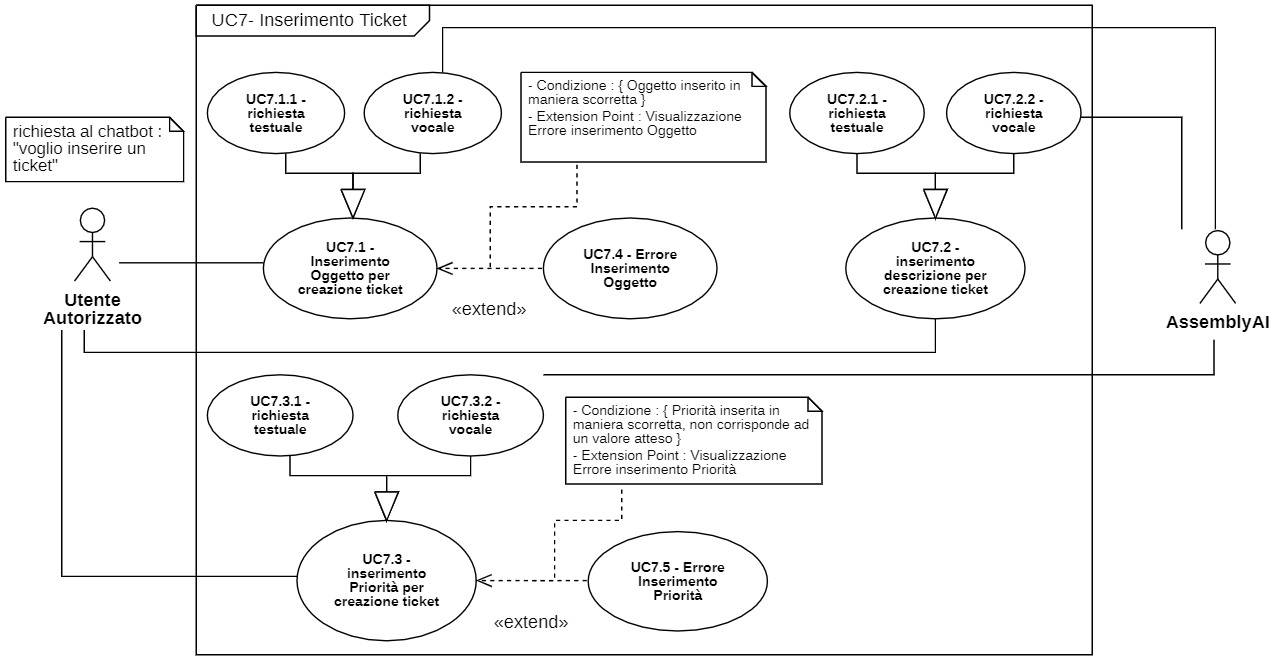
\includegraphics[scale=0.80]{images/UC7.png} 
        \caption{Descrizione grafica caso d'uso UC7}
    \end{figure}

	\item \textbf{Attori}
	\begin{itemize} 
		\item \textit{Primari}: Utente autorizzato
		\item \textit{Secondari}: Non presenti 
	\end{itemize}
	\item \textbf{Descrizione}: L'utente vuole creare un nuovo \glossario{ticket}. Dopo aver ricevuto la richiesta, il chatbot richiede le informazione necessarie al fine di creare un ticket. Il chatbot potrà dover chiedere ulteriori informazioni mancanti o, in caso di errore, comunicare all'utente l'impossibilità di creazione del \glossario{ticket}.
	\item \textbf{Precondizione}: L'utente ha effettuato il login e si trova nella chat.
	\item \textbf{Postcondizione}: \glossario{Ticket} creato con successo.
	\item \textbf{Scenario principale}: \begin{enumerate}
		\item Utente inserisce un messaggio del tipo "Voglio creare un nuovo Ticket";
		\item Chatbot chiede all'utente l'oggeto del \glossario{ticket}; (UC7.1)
    \item Chatbot chiede all'utente la descrizione; (UC7.2)
		\item Chatbot chiede all'utente la priorità. (UC7.3)
	\end{enumerate}
\end{itemize}


\subsubsection{UC7.1 - Inserimento Oggetto per creazione \glossario{ticket}}
\begin{itemize}
	\item \textbf{Identificativo}: UC7.1
	\item \textbf{Nome}: Inserimento Oggetto per creazione \glossario{ticket} 
	\item \textbf{Attori}
	\begin{itemize} 
		\item \textit{Primari}: Utente autorizzato
		\item \textit{Secondari}: Non presenti
	\end{itemize}
	\item \textbf{Descrizione}: L'utente sta eseguendo il procedimento di creazione di un nuovo \glossario{ticket}. Il chatbot richiede all'utente di inserire un Oggetto. 
	\item \textbf{Precondizione}: L'utente ha iniziato la procedura di creazione di un \glossario{ticket}.
	\item \textbf{Postcondizione}: L'utente ha comunicato al chatbot l'oggetto del nuovo ticket.
	\item \textbf{Scenario principale}: \begin{enumerate}
		\item Chatbot interagisce con l'utente: "Indicare l'oggetto del ticket";
		\item Utente fornisce l'oggetto per la creazione del ticket tramite testo (UC7.1.1) o input vocale (UC7.1.2). 
	\end{enumerate}
	\item \textbf{Estensione}: Utente non ha inserito l'oggetto in maniera idonea per il chatbot. (UC7.4)		
\end{itemize}

\paragraph{UC7.1.1 - Richiesta Testuale}
\begin{itemize}
   \item \textbf{Identificativo}: UC7.1.1
   \item \textbf{Nome}: Richiesta testuale
   \item \textbf{Descrizione grafica}: (approfondita in UC7)
   \item \textbf{Attori}:
   \begin{itemize} 
       \item \textit{Primari}: utente autorizzato
       \item \textit{Secondari}: non presenti
   \end{itemize}
       \item \textbf{Precondizione}: L'utente sta creando un ticket e gli è richiesto l'inserimento di un oggetto.
       \item \textbf{Postcondizione}: L'utente comunica un oggetto e procede con la creazione del ticket. 
    \item \textbf{Scenario principale}: 
       \begin{itemize}
           \item Il chatbot richiede l'inserimento di un oggetto;
           \item l'utente inserisce testualmente un oggetto.
       \end{itemize}
\end{itemize}

\paragraph{UC7.1.2 - Richiesta Vocale}
\begin{itemize}
   \item \textbf{Identificativo}: UC7.1.2
   \item \textbf{Nome}: Richiesta Vocale
   \item \textbf{Descrizione grafica}: (approfondita in UC7)
   \item \textbf{Attori}:
   \begin{itemize} 
       \item \textit{Primari}: utente autorizzato
       \item \textit{Secondari}: non presenti
   \end{itemize}
       \item \textbf{Precondizione}: L'utente sta creando un ticket e gli è richiesto l'inserimento di un oggetto.
       \item \textbf{Postcondizione}: L'utente comunica un oggetto e procede con la creazione del ticket. 
    \item \textbf{Scenario principale}: 
       \begin{itemize}  
        \item Il chatbot richiede l'inserimento di un oggetto;
        \item l'utente inserisce vocalmente un oggetto.
       \end{itemize}
\end{itemize}


\subsubsection{UC7.2 - Inserimento descrizione per creazione \glossario{ticket}}
\begin{itemize}
	\item \textbf{Identificativo}: UC7.2
	\item \textbf{Nome}: Inserimento descrizione per creazione \glossario{ticket} 
	\item \textbf{Attori}
	\begin{itemize} 
		\item \textit{Primari}: Utente autorizzato
		\item \textit{Secondari}: Non presenti
	\end{itemize}
	\item \textbf{Descrizione}:  Utente sta eseguendo il procedimento di creazione di un nuovo \glossario{ticket}. Il chatbot richiede all'utente di inserire una descrizione. 
	\item \textbf{Precondizione}: Utente ha comunicato al chatbot l'oggetto del nuovo ticket.
	\item \textbf{Postcondizione}: Utente ha comunicato al chatbot la descrizione del nuovo ticket.
	\item \textbf{Scenario principale}: \begin{enumerate}
		\item Chatbot interagisce con l'utente: "Indicare la descrizione del ticket";
		\item Utente fornisce la descrizione per la creazione del ticket tramite testo (UC7.2.1) o input vocale (UC7.2.2).
	\end{enumerate}
	\end{itemize}

  \paragraph{UC7.2.1 - Richiesta Testuale}
  \begin{itemize}
     \item \textbf{Identificativo}: UC7.2.1
     \item \textbf{Nome}: Richiesta testuale
     \item \textbf{Descrizione grafica}: (approfondita in UC7)
     \item \textbf{Attori}:
     \begin{itemize} 
         \item \textit{Primari}: utente autorizzato
         \item \textit{Secondari}: non presenti
     \end{itemize}
         \item \textbf{Precondizione}: L'utente sta creando un ticket, ha inserito un oggetto e gli è richiesto l'inserimento di una descrizione.
         \item \textbf{Postcondizione}: L'utente comunica una descrizione e procede con la creazione del ticket. 
      \item \textbf{Scenario principale}: 
         \begin{itemize}
             \item Il chatbot richiede l'inserimento di una descrizione;
             \item l'utente inserisce testualmente una descrizione.
         \end{itemize}
  \end{itemize}
  
  \paragraph{UC7.2.2 - Richiesta Vocale}
  \begin{itemize}
     \item \textbf{Identificativo}: UC7.2.2
     \item \textbf{Nome}: Richiesta testuale
     \item \textbf{Descrizione grafica}: (approfondita in UC7)
     \item \textbf{Attori}:
     \begin{itemize} 
         \item \textit{Primari}: utente autorizzato
         \item \textit{Secondari}: non presenti
     \end{itemize}
         \item \textbf{Precondizione}: L'utente sta creando un ticket, ha inserito un oggetto e gli è richiesto l'inserimento di una descrizione.
         \item \textbf{Postcondizione}: L'utente comunica una descrizione e procede con la creazione del ticket. 
      \item \textbf{Scenario principale}: 
         \begin{itemize}  
          \item Il chatbot richiede l'inserimento di una descrizione;
          \item l'utente inserisce vocalmente una descrizione.
         \end{itemize}
  \end{itemize}


  \subsubsection{UC7.3 - Inserimento priorità per creazione \glossario{ticket}}
\begin{itemize}
	\item \textbf{Identificativo}: UC7.3
	\item \textbf{Nome}: Inserimento priorità per creazione \glossario{ticket}
	\item \textbf{Attori}
	\begin{itemize} 
		\item \textit{Primari}: Utente autorizzato
		\item \textit{Secondari}: Non presenti
	\end{itemize}
	\item \textbf{Descrizione}: L'utente sta eseguendo il procedimento di creazione di un nuovo \glossario{ticket}. Il chatbot richiede all'utente di assegnare una priorità.
	\item \textbf{Precondizione}: l'utente ha comunicato al chatbot la priorità del nuovo ticket.
	\item \textbf{Postcondizione}: l'utente ha comunicato al chatbot la priorità del nuovo ticket.
	\item \textbf{Scenario principale}: \begin{enumerate}
		\item Chatbot interagisce con l'utente: "Assegnare una priorità al ticket";
		\item Utente assegna una priorità al ticket tramite testo (UC7.4.1) o input vocale (UC7.4.2).
	\end{enumerate}
	\item \textbf{Estensione}: L'utente non ha inserito la priorità in maniera idonea per il chatbot. (UC7.5)
\end{itemize}

\paragraph{UC7.3.1 - Richiesta Testuale}
\begin{itemize}
   \item \textbf{Identificativo}: UC7.3.1
   \item \textbf{Nome}: Richiesta testuale
   \item \textbf{Descrizione grafica}: (approfondita in UC7)
   \item \textbf{Attori}:
   \begin{itemize} 
       \item \textit{Primari}: utente autorizzato
       \item \textit{Secondari}: non presenti
   \end{itemize}
       \item \textbf{Precondizione}: L'utente sta creando un ticket e gli è richiesto l'inserimento di una priorità.
       \item \textbf{Postcondizione}: L'utente comunica una priorità e viene creato il ticket. 
    \item \textbf{Scenario principale}: 
       \begin{itemize}
           \item Il chatbot richiede l'inserimento di una priorità;
           \item l'utente inserisce testualmente una priorità.
       \end{itemize}
\end{itemize}

\paragraph{UC7.3.2 - Richiesta Vocale}
\begin{itemize}
   \item \textbf{Identificativo}: UC7.3.2
   \item \textbf{Nome}: Richiesta Vocale
   \item \textbf{Descrizione grafica}: (approfondita in UC7)
   \item \textbf{Attori}:
   \begin{itemize} 
       \item \textit{Primari}: utente autorizzato
       \item \textit{Secondari}: non presenti
   \end{itemize}
   \item \textbf{Precondizione}: L'utente sta creando un ticket e gli è richiesto l'inserimento di una priorità.
   \item \textbf{Postcondizione}: L'utente comunica una priorità e viene creato il ticket. 
    \item \textbf{Scenario principale}: 
       \begin{itemize}  
        \item Il chatbot richiede l'inserimento di una priorità;
        \item l'utente inserisce vocalmente una priorità.
       \end{itemize}
\end{itemize}

\subsubsection{UC7.4 - Visualizzazione errore inserimento oggetto}
\begin{itemize}
	\item \textbf{Identificativo}: UC7.4
	\item \textbf{Nome}: Visualizzazione errore inserimento oggetto 
	\item \textbf{Attori}
	\begin{itemize} 
		\item \textit{Primari}: Utente autorizzato
		\item \textit{Secondari}: Non presenti
	\end{itemize}
	\item \textbf{Descrizione}: È avvenuto un errore nell'inserimento dell'oggetto. Il chatbot mostra l'errore all'utente.
	\item \textbf{Precondizione}: L'utente sta eseguendo l'operazione di inserimento di un nuovo ticket. L'oggetto risulta essere inserito in un formato non valido. 
	\item \textbf{Postcondizione}: Il chatbot mostra all'utente che l'oggetto non è stato inserito in maniera idonea per il chatbot.
	\item \textbf{Scenario principale}: \begin{enumerate}
		\item Chatbot mostra all'utente che è avvenuto un errore tramite chat: "Oggetto inserito in maniera non idonea".
		\end{enumerate}
\end{itemize}


\subsubsection{UC7.5 - Visualizzazione errore inserimento priorità}
\begin{itemize}
	\item \textbf{Identificativo}: UC7.5
	\item \textbf{Nome}:  Visualizzazione errore inserimento priorità
	\item \textbf{Attori}
	\begin{itemize} 
		\item \textit{Primari}: Utente autorizzato
		\item \textit{Secondari}: Non presenti
	\end{itemize}
	\item \textbf{Descrizione}: È avvenuto un errore nell'inserimento della priorità. Il chatbot mostra l'errore all'utente.
	\item \textbf{Precondizione}: L'utente sta eseguendo l'operazione di inserimento di un nuovo ticket. La priorità risulta essere inserita in un formato non valido. 
	\item \textbf{Postcondizione}: Il chatbot mostra all'utente che la priorità non è stata inserita in maniera idonea per il chatbot o non assume uno dei valori fissi che il chatbot si aspetta.
	\item \textbf{Scenario principale}: \begin{enumerate}
		\item Chatbot mostra all'utente che è avvenuto un errore tramite chat: "Priorità inserita in maniera non idonea".
	\end{enumerate}
\end{itemize}
\newpage